\documentclass[11pt]{article}
\usepackage{preamble}
\usepackage[]{gset}
\def\week{9}
\def\theproblem{К\week.\arabic{problem}}


\def\FN{\mathcal{N}_f}
\begin{document}
	\setcounter{problem}{0}
	\def\theproblem{Д\week.\arabic{problem}}
	{\textbf{\large Дискретная математика}\hfill \textbf{(Основной поток)}
		
		\medskip %
		
		\textbf{Домашнее задание \week}}
	
	\medskip
	
	\textbf{Дайте обоснованные ответы на следующие вопросы.}
	
	
	\vspace{5mm}
	
	
	
	\p Существует ли  граф на 10 вершинах, степени которых равны $1,1,1,1,1,1,3,5,5,5$?
	
	\[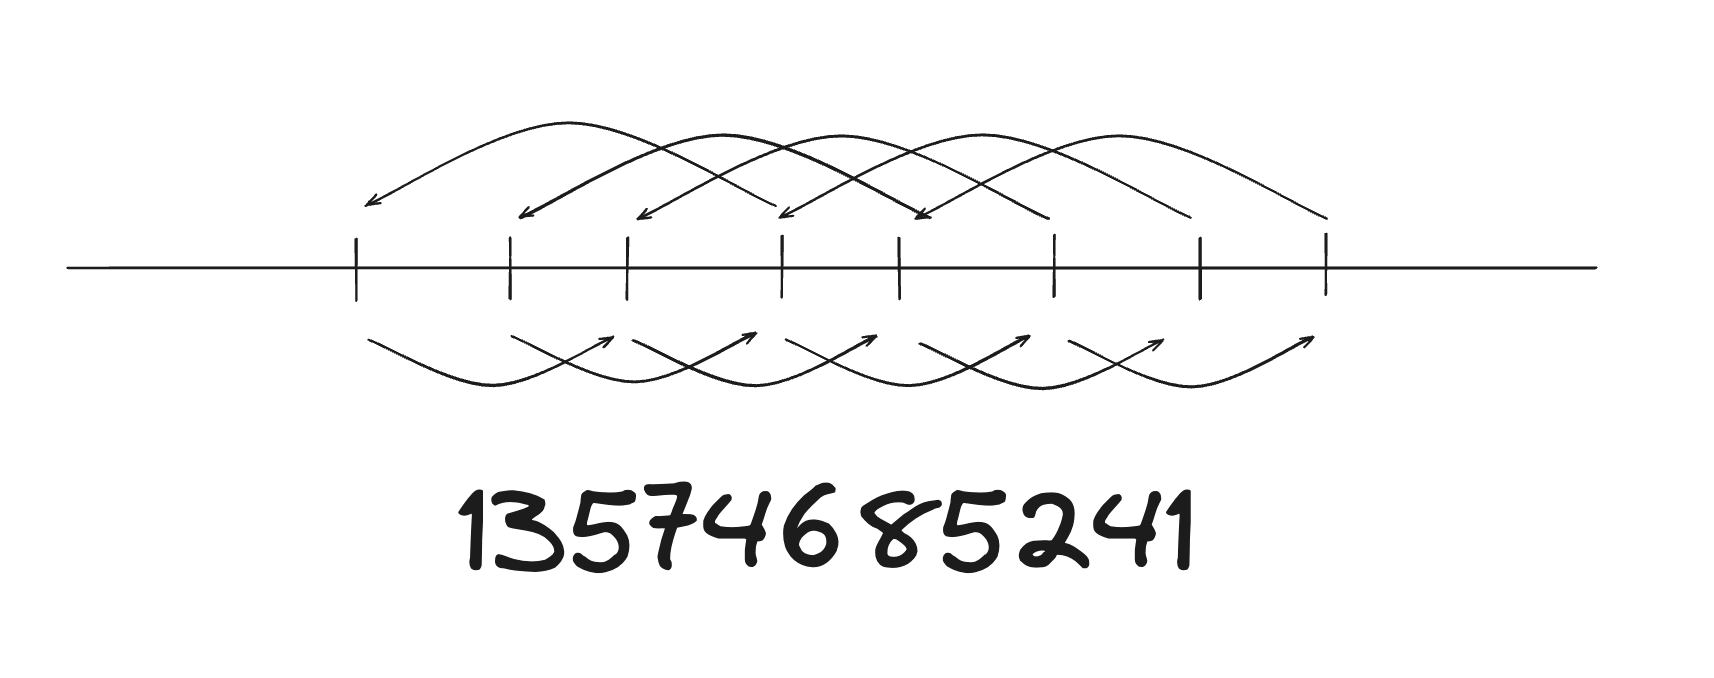
\includegraphics[width=150mm]{img}\]
	
	\p Найдите наименьшее количество вершин в  графе,  сумма степеней
	вершин в котором равна~26.
	
	Наименьшее количество вершин для заданного числа ребер в полном графе. Ребер в данном графе $\frac{26}{2} = 13$. В полном графе наибольшее количество ребер для заданного числа вершин. В полном графе на 5 вершинах $\frac{5*4}{2} = 10$ ребер, значит вершин больше 5. Ребер в полном графе на 6 вершинах $\frac{6*5}{2} = 15$, что больше 13, то есть можно убрать 2 ребра и получить граф из условия на 6 вершинах. 
	
	\answer{6} \sspace
	
	\p Вершины графа $G$~"--- слова длины 2 в алфавите
	$\{0,1,2,3,4,5,6,7,8,9\}$, то есть последовательности десятичных цифр
	длины~2. Две вершины (два слова длины~2) соединены ребром в~$G$, если
	в каждой из позиций цифры различаются ровно на~1. Найдите количество компонент связности графа~$G$.
	
	Заметим, что при переходе по ребрам не меняется остаток от деления суммы цифр числа на 2. Это значит, что существует как минимум 2 компоненты связности. Докажем, что компонент связности ровно 2. Опишем путь внутри одной компоненты связности. Пусть $\overline{ab}$ и $\overline{cd}$ находятся внутри одной компоненты связности. В этой задаче пару чисел $(A, B)$ я буду называть ребром, если оно переводит из числа $\overline{x , y}$ в число $\overline{x + A, y + B}$. Под суммой ребер я подразумеваю постепенное прохождение по ребрам. Мы хотим получить сумму ребер, которая будет равна ребру $(c - a, d - b)$. Важно заметить, что так как $a + b \equiv c + d \mod 2$, то $c - a \equiv d - b \mod 2$. Покажем, что любое подобное ребро можно получить комбинацией имеющихся.  Можем получить ребро $(2, 0)$, как $(1, 1)+(1, -1)$ или $(1, -1)+(1, 1)$. Аналогично для любого числа можно получить ребра $(-2, 0), (0, 2), (0, -2)$. Получается, что можно получить любое ребро $(2k, 2n)$, где $k, n \in \{-4,-3,-2,-1,0,1,2,3,4\}.$ Теперь, применив одно из ребер $(-1, -1), (1, 1)$ - можно получить любое ребро, где 2 числа его определяющие одной четности. Получается, что можно получить и ребро $(c - a, d - b)$, значит существует путь между $\overline{ab}$ и $\overline{cd}$.  \sspace
		
	\p Пусть $A$~"--- непустое множество,  $E_1$ и $E_2$~"---  такие отношения эквивалентности на $A$, что $E_1\cup E_2$ также является отношением эквивалентности, $C_1$~"--- класс эквивалентности отношения $E_1$, $C_2$~"--- класс эквивалентности отношения $E_2$. Докажите, что $C_1\cap C_2 = \es$, или $C_1\subseteq C_2$, или $C_2\subseteq C_1$.
	
	Пусть $C_1(x) \cap C_2(y) \neq \es \Rightarrow \forall z \in C_2 (x, z) \in E_1 \cup E_2$ 
\end{document}